
\documentclass[a4paper,12pt]{article}
\usepackage{epstopdf}
\usepackage[utf8]{inputenc}
\usepackage[english]{babel}
\usepackage{enumerate}
\usepackage{mathtools}
\usepackage{hyperref}
\usepackage{float}
\usepackage[pdftex]{graphicx}   
\usepackage{multirow}
\usepackage{listings}
\lstset{
    language=matlab,
    basicstyle=\ttfamily
}

\title{TBMI26  \\
       Assignment 2}
\author{Martin Estgren \texttt{<mares480>}}
      
\begin{document}
 \pagenumbering{arabic}
    \maketitle % Generate.

\section{Boosting using the AdaBoost algorithm}

For the test we examine the performance of cascaded haar-classifiers from a single one up to \textit{200}. We use \textit{400} samples for training set, that is \textit{200} images of faces and \textit{200} of non-faces. For the testing/validation dataset we use \textit{200} images, \textit{100} faces and \textit{100} non-faces. 

\begin{figure}[H]
\centering
\caption{Sample of non-faces respective faces}\label{fig:sample_data_set}
  \begin{minipage}[]{0.8\textwidth}
  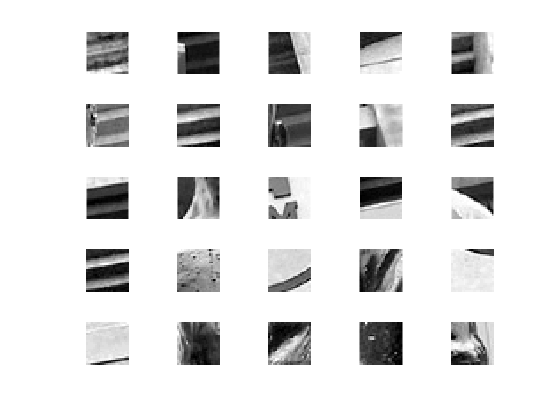
\includegraphics[width=\textwidth]{figures/sample_of_non_faces.png}
  \end{minipage}
    \begin{minipage}[]{0.8\textwidth}
  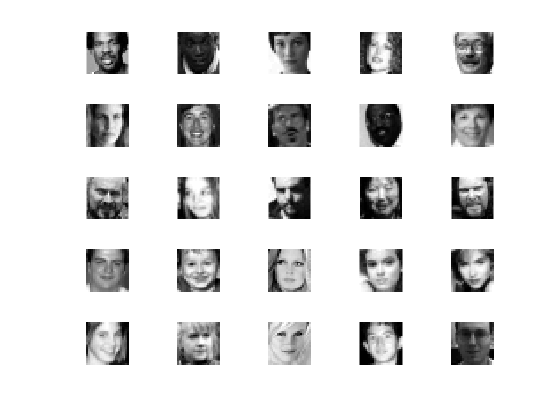
\includegraphics[width=\textwidth]{figures/sample_of_faces.png}
  \end{minipage}
\end{figure}
\begin{figure}[H]
\centering
\caption{Sample of haar-features}\label{fig:sample_haar_features}
  \begin{minipage}[]{0.8\textwidth}
  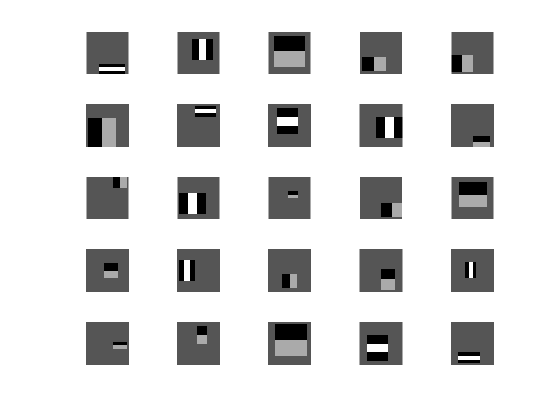
\includegraphics[width=\textwidth]{figures/sample_of_haar_features.png}
  \end{minipage}
\end{figure}

Below we can observe the error in accuracy given the number of weak classifiers for the training. When we increase the number of classifiers the correct classification rate increases. Looking only at the training data we pick 340 as the best number of classifiers.
\begin{figure}[H]
\centering
\caption{Training error given the number of weak classifiers}\label{fig:train_error}
  \begin{minipage}[]{0.80\textwidth}
  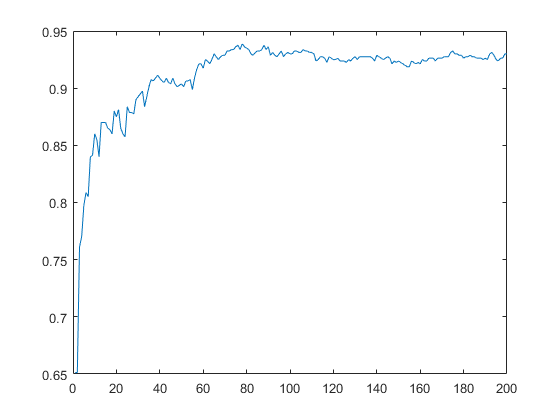
\includegraphics[width=\textwidth]{figures/train_error.png}
  \end{minipage}
\end{figure}

Below we can observe the error in accuracy given the number of weak classifiers for the test data. When we increase the number of classifiers the correct classification rate doesn't necessarily increase. increases. When we also consider the testing data set we pick \textit{74} as the best number of classifiers with an accuracy of \textit{0.9125}.

\begin{figure}[H]
\centering
\caption{Test error given the number of weak classifiers}\label{fig:test_error}
  \begin{minipage}[]{0.80\textwidth}
  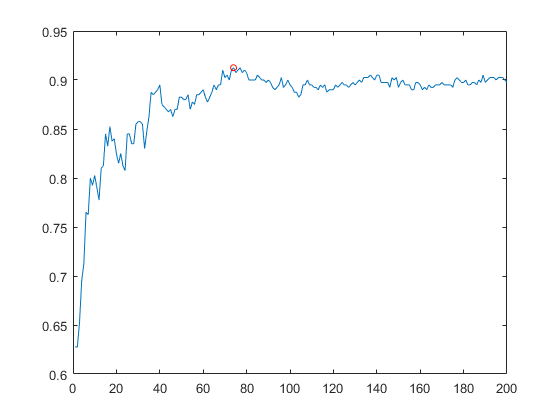
\includegraphics[width=\textwidth]{figures/test_error.png}
  \end{minipage}
\end{figure}

Below we have two plots of faces and non-faces respectively that was hard to classify. Over all we can see how low-contrast makes it harder to classify an image. This is a reasonable assumption given that we work with small gradients as weak-classifiers.

\begin{figure}[H]
\centering
\caption{Misclassified images}\label{fig:missclassified_faces}
  \begin{minipage}[]{0.8\textwidth}
  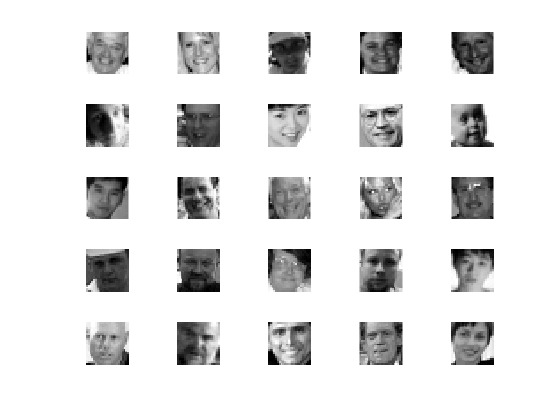
\includegraphics[width=\textwidth]{figures/missclassified_faces.png}
  \end{minipage}
    \begin{minipage}[]{0.8\textwidth}
  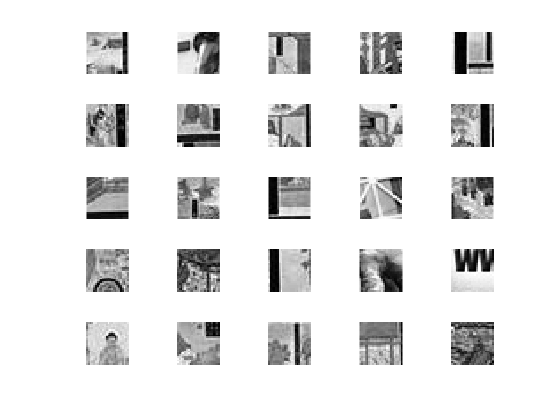
\includegraphics[width=\textwidth]{figures/missclassified_non_faces.png}
  \end{minipage}
\end{figure}

\end{document}
